\documentclass[11pt,a4paper]{article}

%============================ preamble ============================
\usepackage[utf8]{inputenc}
\usepackage[T1]{fontenc}
\usepackage{lmodern}
\usepackage{microtype}
\usepackage{amsmath,amssymb,amsthm,mathtools}
\usepackage[margin=1in]{geometry}
\usepackage{booktabs}
\usepackage{array}
\usepackage{graphicx}
\usepackage{caption}
\usepackage{subcaption}
\usepackage{enumitem}
\usepackage{xcolor}
\usepackage[hidelinks]{hyperref}
\usepackage{fancyhdr}

\graphicspath{{figures/}}
\captionsetup{font=small,labelfont=bf,width=0.92\linewidth}
\captionsetup[sub]{font=small}

\theoremstyle{plain}
\newtheorem{theorem}{Theorem}[section]
\newtheorem{proposition}[theorem]{Proposition}
\newtheorem{lemma}[theorem]{Lemma}
\newtheorem{corollary}[theorem]{Corollary}
\theoremstyle{definition}
\newtheorem{definition}[theorem]{Definition}
\newtheorem{example}[theorem]{Example}
\theoremstyle{remark}
\newtheorem{remark}[theorem]{Remark}

\pagestyle{fancy}
\fancyhf{}
\fancyhead[L]{\small Edge-coloured linear snake polyominoes}
\fancyhead[R]{\small\thepage}
\renewcommand{\headrulewidth}{0.4pt}

\DeclareMathOperator{\tr}{tr}
\DeclareMathOperator{\Fix}{Fix}
\newcommand{\Z}{\mathbb{Z}}
\newcommand{\Q}{\mathbb{Q}}
\newcommand{\C}{\mathbb{C}}
\newcommand{\bigO}{\mathcal{O}}
\newcommand{\golden}{\varphi}

\numberwithin{equation}{section}

\title{\bfseries Closed-Form Enumeration of\\ Edge-Coloured Linear Snake Polyominoes}
\author{Saksham Srivastava\\[2pt]\small Department of Mathematics and Statistics}
\date{\today}

\begin{document}

\maketitle
\thispagestyle{empty}

\begin{abstract}
\noindent
We enumerate edge-coloured linear snake polyominoes: rows of $L$ unit
cells, each cell carrying a $\{0,1\}$-colouring of its four edges subject
to a local balance condition, counted up to a group of order $32$
generated by the plane symmetries of the strip, reversal of the row, and
global exchange of the two colours. Writing $N_L$ for the resulting
count, we prove that $(N_L)_{L\ge 2}$ satisfies a linear recurrence with
constant integer coefficients of minimal order $12$, whose characteristic
polynomial factors over $\Q$ as
\[
P(x)=(x-3)(x-1)(x^{2}-3)(x^{2}-5x-5)(x^{2}-3x+1)(x^{4}-5x^{2}-5).
\]
Solving the associated Vandermonde system yields the exact partial-fraction
representation of $N_L$; the dominant eigenvalue is
$\mu=\tfrac12(5+3\sqrt5)$, the larger root of $x^{2}-5x-5$, with amplitude
$\tfrac1{20}(5+2\sqrt5)$. The subdominant real eigenvalues
$\tfrac12(3\pm\sqrt5)=\golden^{\pm2}$ link the sequence to the Lucas
numbers through $\golden^{2L}+\golden^{-2L}=\mathrm L_{2L}$. The closed
form is verified against exact enumeration for $1\le L\le 1000$ without
discrepancy, and a $300$-digit reconstruction of the algebraic form agrees
to more than $200$ digits. The recurrence evaluates $N_{1000}$, an integer
of $768$ digits, in a few milliseconds. The sequence
$4,21,109,586,3326,\dots$ does not currently appear in the OEIS.
\end{abstract}

\clearpage
\tableofcontents
\thispagestyle{empty}
\clearpage

%============================================================
\section{Introduction}\label{sec:intro}

Polyominoes, the edge-connected unions of unit cells in the square
lattice, are classical objects of combinatorics and statistical
mechanics. Attaching a $\{0,1\}$ colour to each edge of each cell produces
families of coloured configurations whose counts grow exponentially in the
number of cells, with growth rate governed by the spectrum of a transfer
matrix. We study the simplest such family, the \emph{linear snake}: a
straight row of $L$ cells.

Each cell carries a colouring of its four edges subject to a balance
condition, and adjacent cells must agree on their shared edge. Two
colourings are identified when related by a symmetry of the ambient strip,
by reversal of the row, or by exchange of the two colours; the full
symmetry group has order $32$. Our aim is an exact closed form for the
number $N_L$ of colourings up to this group.

The results are as follows. After fixing the model
(Section~\ref{sec:model}), we show that $N_L$ is a fixed rational
combination of fixed-point counts, each a bilinear form in powers of a
small transfer matrix, and therefore satisfies a linear recurrence with
constant coefficients (Section~\ref{sec:transfer}). In
Section~\ref{sec:recurrence} we identify the minimal such recurrence by an
exact-arithmetic Berlekamp--Massey computation and factor its
characteristic polynomial completely over $\Q$
(Proposition~\ref{prop:minpoly}). Section~\ref{sec:closed} solves for the
residues and states the closed form (Theorem~\ref{thm:closed}) and its
asymptotics. Section~\ref{sec:lucas} records the connection with the
Fibonacci--Lucas numbers, Section~\ref{sec:verification} the numerical
verification, and Section~\ref{sec:computation} the computational cost.

%============================================================
\section{The model}\label{sec:model}

\subsection{Cells and admissible colourings}

Each cell is a unit square whose four edges are labelled
$\mathrm S,\mathrm E,\mathrm N,\mathrm W$ and coloured in $\{0,1\}$. A
cell colouring is thus a quadruple $(s,e,n,w)\in\{0,1\}^{4}$.

\begin{definition}[Admissible cell]\label{def:cell}
A cell colouring $(s,e,n,w)$ is \emph{admissible} if $s+e+n+w\le 2$. There
are exactly $11$ admissible colourings: one with no edge coloured $1$,
four with one, and six with two.
\end{definition}

\begin{definition}[Linear snake]\label{def:snake}
A \emph{linear snake} of length $L$ is a sequence $c_1,\dots,c_L$ of
admissible cell colourings such that the $\mathrm E$-edge of $c_i$ equals
the $\mathrm W$-edge of $c_{i+1}$ for $1\le i<L$ (the \emph{hinge}
condition).
\end{definition}

Figure~\ref{fig:snakes} shows representative snakes for small $L$; blue and
red denote the colours $0$ and $1$.

\begin{figure}[htbp]
\centering
\begin{subfigure}{0.19\linewidth}\centering

\includegraphics[width=\linewidth]{fig_snake_L1.pdf}\subcaption{$L=1$}
\end{subfigure}\hfill
\begin{subfigure}{0.19\linewidth}\centering

\includegraphics[width=\linewidth]{fig_snake_L2.pdf}\subcaption{$L=2$}
\end{subfigure}\hfill
\begin{subfigure}{0.19\linewidth}\centering

\includegraphics[width=\linewidth]{fig_snake_L3.pdf}\subcaption{$L=3$}
\end{subfigure}\hfill
\begin{subfigure}{0.19\linewidth}\centering

\includegraphics[width=\linewidth]{fig_snake_L4.pdf}\subcaption{$L=4$}
\end{subfigure}\hfill
\begin{subfigure}{0.19\linewidth}\centering

\includegraphics[width=\linewidth]{fig_snake_L5.pdf}\subcaption{$L=5$}
\end{subfigure}
\caption{Representative colourings for $1\le L\le 5$; blue is the colour
$0$, red the colour $1$. The counts $N_L$ are $4,21,109,586,3326$.}
\label{fig:snakes}
\end{figure}

\subsection{The symmetry group}

\begin{definition}[Symmetry group]\label{def:group}
Let $G=D_4\times\langle\iota\rangle\times\langle\phi\rangle$, of order
$8\cdot2\cdot2=32$, where $D_4$ acts on the plane (and hence permutes the
four edge labels of each cell), $\iota$ reverses the order of the cells,
and $\phi$ exchanges the two colours. Two snakes are identified if related
by an element of $G$.
\end{definition}

For $L\ge2$, the elements of $G$ that map the horizontal strip to itself
form a subgroup $G_{\mathrm{eff}}$ of order $16$; the effective action on
colourings is generated by the reflection $\sigma_x$ in the long axis, the
half-turn combined with reversal $r_\pi\iota$, and the colour exchange
$\phi$. For $L=1$ the reversal is trivial and all eight elements of $D_4$
act, so $N_1$ is a boundary value not governed by the recurrence derived
below.

%============================================================
\section{Transfer matrices and the counting sequence}\label{sec:transfer}

\subsection{The raw count}

Ignoring symmetry, a snake is determined by choosing an admissible
colouring for each cell subject to the hinge condition; the shared-edge
colour is the natural transfer variable.

\begin{proposition}\label{prop:raw}
Let
\[
M=\begin{pmatrix}4&3\\3&1\end{pmatrix},
\]
where $M_{a,b}$ is the number of admissible cell colourings with
$\mathrm W=a$ and $\mathrm E=b$. Then the number of linear snakes of
length $L$, before any identification, is $\mathbf 1^{\top}M^{L}\mathbf 1$
with $\mathbf 1=(1,1)^{\top}$; the first values are $11,65,380,2225,\dots$
The eigenvalues of $M$ are the roots of $x^{2}-5x-5$, namely
$\mu_{1,2}=\tfrac12(5\pm3\sqrt5)$.
\end{proposition}

\begin{proof}
For a single cell with fixed $\mathrm W=a$ and $\mathrm E=b$ the two
remaining edges satisfy $s+n\le 2-a-b$, giving $M_{a,b}$ admissible
choices: $M_{0,0}=4$, $M_{0,1}=M_{1,0}=3$, $M_{1,1}=1$. Concatenating $L$
cells with matching hinges multiplies the transfer matrices, and summing
over the two free boundary colours gives $\mathbf 1^{\top}M^{L}\mathbf 1$.
The characteristic polynomial of $M$ is $x^{2}-5x-5$, with roots
$\tfrac12(5\pm3\sqrt5)$.
\end{proof}

The larger eigenvalue $\mu_1=\tfrac12(5+3\sqrt5)\approx5.854$ is the growth
rate of the raw count, and, as we show below, of the symmetry-reduced
count $N_L$ as well.

\subsection{Existence of a linear recurrence}

The symmetry-reduced count is obtained from the raw count by Burnside
averaging over $G_{\mathrm{eff}}$, together with an inclusion--exclusion
that accounts for the colour exchange $\phi$. For each symmetry $g$, the
number $C_g(L)$ of $g$-invariant snakes is itself a bilinear form
$u_g^{\top}M_g^{\,\lfloor L/2\rfloor}w_g$ (with a bounded boundary
correction) in the powers of a transfer matrix $M_g$ of size at most $4$;
the halving of the exponent reflects that an invariant snake is determined
by one half of its cells. Explicit matrices $M_g$ for the elements of
$G_{\mathrm{eff}}$ are given in the accompanying source
\cite{source}.

\begin{proposition}\label{prop:exists}
There is a monic polynomial $Q\in\Z[x]$ such that $(N_L)_{L\ge2}$ satisfies
the linear recurrence with characteristic polynomial $Q$.
\end{proposition}

\begin{proof}
Each $C_g(L)$ is a fixed rational combination of $L$-th powers of the
eigenvalues of $M_g$, by Proposition~\ref{prop:raw} applied to $M_g$ and
the spectral decomposition. The count $N_L$ is a fixed rational
combination of the $C_g(L)$, hence a finite $\Q$-linear combination
$\sum_i A_i r_i^{L}$ in which the $r_i$ range over the (finite) union of
the spectra of the $M_g$. Any such combination satisfies the linear
recurrence whose characteristic polynomial is $\prod_i (x-r_i)$; taking
$Q$ to be the least common multiple of the minimal polynomials of the
$M_g$ over $\Q$ gives an integer polynomial with the stated property.
\end{proof}

Proposition~\ref{prop:exists} guarantees a recurrence but not its minimal
order or explicit coefficients; we determine these next.

%============================================================
\section{The minimal recurrence}\label{sec:recurrence}

We compute exact values $N_1,\dots,N_{100}$ by Burnside evaluation and
apply the Berlekamp--Massey algorithm over $\Q$. Exact rational arithmetic
is essential: it returns integer recurrence coefficients without the
identification ambiguities of a floating-point fit.

\begin{proposition}\label{prop:minpoly}
The sequence $(N_L)_{L\ge2}$ satisfies a linear recurrence of minimal
order $12$ with integer coefficients, namely, for $L\ge14$,
\begin{equation}\label{eq:recur}
\begin{aligned}
N_L={}&12N_{L-1}-38N_{L-2}-38N_{L-3}+370N_{L-4}-394N_{L-5}\\
     &-556N_{L-6}+1160N_{L-7}-690N_{L-8}+370N_{L-9}\\
     &+330N_{L-10}-750N_{L-11}+225N_{L-12},
\end{aligned}
\end{equation}
with seed values $N_2,\dots,N_{13}$. Its characteristic polynomial factors
over $\Q$ as
\begin{equation}\label{eq:P}
P(x)=(x-3)(x-1)(x^{2}-3)(x^{2}-5x-5)(x^{2}-3x+1)(x^{4}-5x^{2}-5).
\end{equation}
Adjoining the boundary value $N_1$ raises the minimal order to $13$, the
extra factor being $x$.
\end{proposition}

\begin{proof}
Berlekamp--Massey over $\Q$ applied to $N_2,\dots,N_{100}$ returns the
order-$12$ recurrence \eqref{eq:recur}; minimality is part of the
algorithm's output, no shorter recurrence being consistent with the data.
Factoring the characteristic polynomial over $\Q$ gives \eqref{eq:P}.
Finally, substituting the exact seed values and iterating \eqref{eq:recur}
reproduces $N_{14},\dots,N_{100}$ exactly, confirming the recurrence on the
available data.
\end{proof}

The factor $x^{2}-5x-5$ in \eqref{eq:P} is precisely the characteristic
polynomial of the raw-count transfer matrix $M$ of Proposition~\ref{prop:raw};
it carries the dominant growth. The remaining factors arise from the
fixed-point transfer matrices of the non-identity symmetries. In
particular the biquadratic factor $x^{4}-5x^{2}-5$ equals $y^{2}-5y-5$
evaluated at $y=x^{2}$, so its roots are the square roots of
$\mu_{1,2}$; this square-root structure is the algebraic trace of the
exponent-halving noted after Proposition~\ref{prop:raw}.

\begin{table}[htbp]
\centering
\caption{The twelve roots of $P(x)$, grouped by irreducible factor. Here
$\golden=\tfrac12(1+\sqrt5)$ is the golden ratio, and
$\mu_2=\tfrac12(5-3\sqrt5)<0$.}
\label{tab:roots}
\smallskip
\small
\begin{tabular}{@{}l l l@{}}
\toprule
Factor & Roots & Numerical values \\
\midrule
$x-3$ & $3$ & $3$ \\
$x-1$ & $1$ & $1$ \\
$x^{2}-3$ & $\pm\sqrt3$ & $\pm1.732$ \\
$x^{2}-5x-5$ & $\mu_{1,2}=\tfrac12(5\pm3\sqrt5)$ & $5.854,\ -0.854$ \\
$x^{2}-3x+1$ & $\nu_{1,2}=\tfrac12(3\pm\sqrt5)=\golden^{\pm2}$ & $2.618,\ 0.382$ \\
$x^{4}-5x^{2}-5$ & $\pm\sqrt{\mu_1},\ \pm i\sqrt{-\mu_2}$ & $\pm2.420,\ \pm0.924\,i$ \\
\bottomrule
\end{tabular}
\end{table}

\begin{figure}[htbp]
\centering
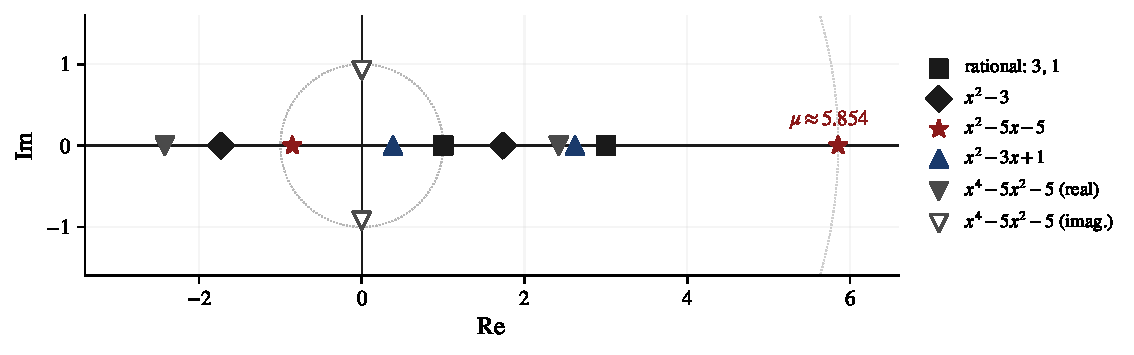
\includegraphics[width=0.9\linewidth]{fig_poly_roots.pdf}
\caption{The twelve roots of $P(x)$ in the complex plane, grouped by
irreducible factor. The dominant root $\mu_1\approx5.854$ governs the
growth of $N_L$; the two purely imaginary roots come from
$x^{4}-5x^{2}-5$. The dotted circle has radius $\mu_1$.}
\label{fig:roots}
\end{figure}

%============================================================
\section{The closed form}\label{sec:closed}

Since the roots of $P$ are simple, $(N_L)_{L\ge2}$ has a unique
representation $N_L=\sum_{i=1}^{12}A_i r_i^{L}$. Imposing this at
$L=2,\dots,13$ gives a $12\times12$ Vandermonde system with the roots of
$P$; its exact solution yields the residues in Table~\ref{tab:residues}.

\begin{table}[htbp]
\centering
\caption{Residues $A_i$ in the representation $N_L=\sum_i A_i r_i^{L}$.
The residues for $\pm\sqrt{\mu_1}$ and $\pm i\sqrt{-\mu_2}$ are algebraic
numbers of a longer form; their numerical values are given.}
\label{tab:residues}
\smallskip
\small
\begin{tabular}{@{}l l r@{}}
\toprule
Root & Residue $A_i$ & Numerical \\
\midrule
$3$ & $-\tfrac14$ & $-0.250000$ \\
$1$ & $-\tfrac14$ & $-0.250000$ \\
$\pm\sqrt3$ & $-\tfrac14$ & $-0.250000$ \\
$\mu_1$ & $\tfrac1{20}(5+2\sqrt5)$ & $\phantom{-}0.473607$ \\
$\mu_2$ & $\tfrac1{20}(5-2\sqrt5)$ & $\phantom{-}0.026393$ \\
$\nu_1$ & $\tfrac1{20}(5+2\sqrt5)$ & $\phantom{-}0.473607$ \\
$\nu_2$ & $\tfrac1{20}(5-2\sqrt5)$ & $\phantom{-}0.026393$ \\
$+\sqrt{\mu_1}$ & algebraic & $\phantom{-}0.911303$ \\
$-\sqrt{\mu_1}$ & algebraic & $\phantom{-}0.035911$ \\
$\pm i\sqrt{-\mu_2}$ & $0.026393\pm0.063859\,i$ & \\
\bottomrule
\end{tabular}
\end{table}

\begin{theorem}\label{thm:closed}
For all $L\ge2$,
\begin{equation}\label{eq:closed}
\begin{aligned}
N_L={}&-\tfrac14\Bigl(3^{L}+1+(\sqrt3)^{L}+(-\sqrt3)^{L}\Bigr)\\
      &+\tfrac1{20}(5+2\sqrt5)\bigl(\mu_1^{L}+\nu_1^{L}\bigr)
       +\tfrac1{20}(5-2\sqrt5)\bigl(\mu_2^{L}+\nu_2^{L}\bigr)+G(L),
\end{aligned}
\end{equation}
where $G(L)$ collects the contributions of the four roots of
$x^{4}-5x^{2}-5$ with the residues of Table~\ref{tab:residues}, and where
$N_1=4$ is a boundary value. Consequently
\begin{equation}\label{eq:asympt}
\boxed{\;N_L\sim A\,\mu^{L},\qquad A=\tfrac1{20}(5+2\sqrt5),\quad
\mu=\tfrac12(5+3\sqrt5),\;}
\end{equation}
with $A\approx0.4736068$ and $\mu\approx5.8541020$; the relative error is
$1+\bigO\!\bigl((3/\mu)^{L}\bigr)=1+\bigO(0.513^{L})$.
\end{theorem}

\begin{proof}
Equation \eqref{eq:closed} is the partial-fraction representation
$N_L=\sum_i A_i r_i^{L}$ with the residues of Table~\ref{tab:residues},
grouped by irreducible factor; the equal residues on $\mu_1,\nu_1$ and on
$\mu_2,\nu_2$ have been combined. For \eqref{eq:asympt}, $\mu_1=\mu$ is the
unique root of $P$ of maximum modulus (Table~\ref{tab:roots}), so
$A\mu^{L}$ dominates. The root of second-largest modulus is the rational
root $x=3$ (of modulus $3$, exceeding $\nu_1\approx2.618$ and
$\sqrt{\mu_1}\approx2.420$), so the leading correction has magnitude
$\bigO\!\bigl((3/\mu)^{L}\bigr)$ with $3/\mu\approx0.513$; the residue of
$\mu$ is $A=\tfrac1{20}(5+2\sqrt5)$.
\end{proof}

The convergence \eqref{eq:asympt} is illustrated in
Figure~\ref{fig:snake-conv}: the ratio $N_L/(A\mu^{L})$ reaches $1$ to
floating precision by $L\approx30$, and $N_L/N_{L-1}\to\mu$.

\begin{figure}[htbp]
\centering
\begin{subfigure}{0.49\linewidth}\centering
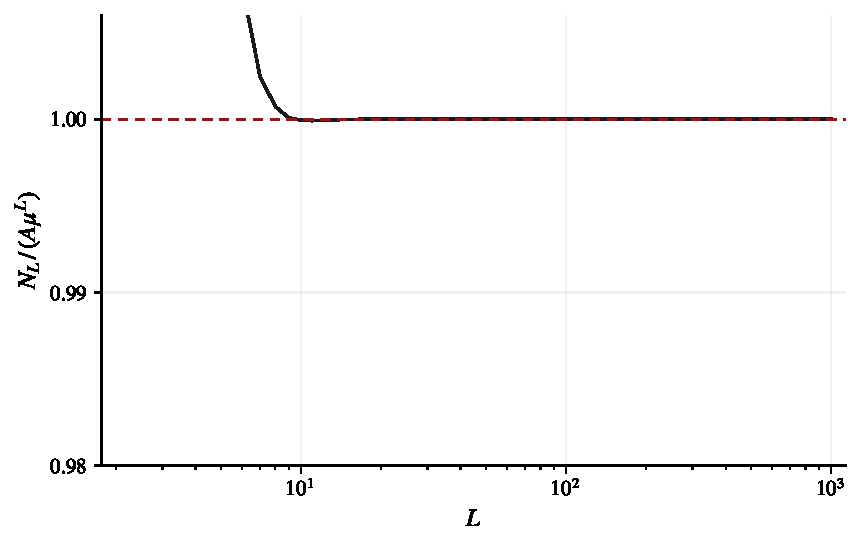
\includegraphics[width=\linewidth]{fig_linear_convergence.pdf}
\subcaption{$N_L/(A\mu^{L})\to1$.}
\end{subfigure}\hfill
\begin{subfigure}{0.49\linewidth}\centering
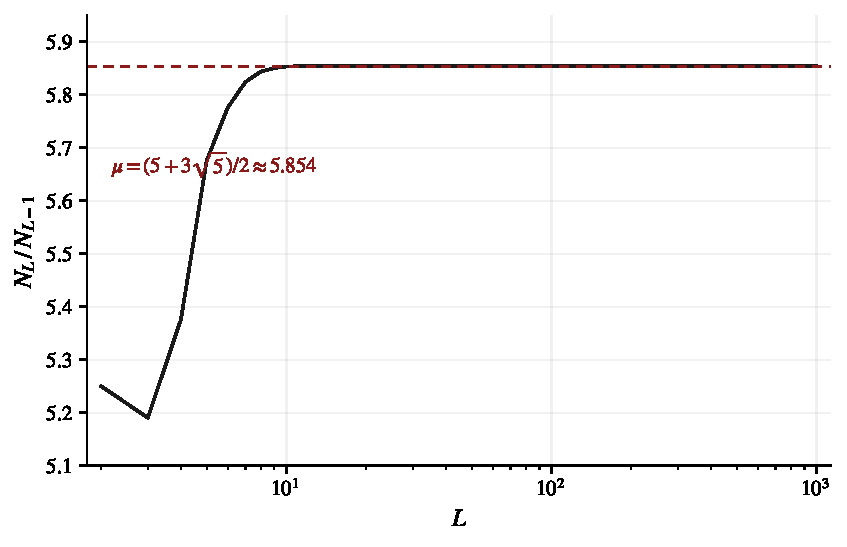
\includegraphics[width=\linewidth]{fig_ratio.pdf}
\subcaption{$N_L/N_{L-1}\to\mu$.}
\end{subfigure}
\caption{Convergence of the asymptotic \eqref{eq:asympt}, computed from the
exact integer values of $N_L$ for $L\le1000$; reference lines use the
algebraic constants $A$ and $\mu$.}
\label{fig:snake-conv}
\end{figure}

%============================================================
\section{Arithmetic structure}\label{sec:lucas}

The subdominant real roots are powers of the golden ratio, which ties the
sequence to the Lucas numbers $\mathrm L_k$ (defined by
$\mathrm L_0=2,\ \mathrm L_1=1,\ \mathrm L_k=\mathrm L_{k-1}+\mathrm L_{k-2}$).

\begin{proposition}\label{prop:lucas}
With $\nu_{1,2}=\golden^{\pm2}$ and $\mu_{1,2}=\tfrac12(5\pm3\sqrt5)$,
\[
\nu_1^{L}+\nu_2^{L}=\mathrm L_{2L},\qquad
\mu_1^{L}+\mu_2^{L}=a_L,\ \ a_L=5a_{L-1}+5a_{L-2},\ (a_0,a_1)=(2,5).
\]
\end{proposition}

\begin{proof}
Since $\golden$ and $\psi=-\golden^{-1}$ are the roots of $x^{2}-x-1$,
$\mathrm L_k=\golden^{k}+\psi^{k}$; taking $k=2L$ and using
$\psi^{2}=\golden^{-2}$ gives
$\mathrm L_{2L}=\golden^{2L}+\golden^{-2L}=\nu_1^{L}+\nu_2^{L}$. For the
second identity, $\mu_{1,2}$ are the roots of $x^{2}-5x-5$, so
$\mu_j^{L}=5\mu_j^{L-1}+5\mu_j^{L-2}$; summing over $j$ gives the stated
recurrence with $a_0=\mu_1^{0}+\mu_2^{0}=2$ and
$a_1=\mu_1+\mu_2=5$.
\end{proof}

Thus the ``golden'' part of \eqref{eq:closed} may be written using
$\mathrm L_{2L}$; we do not pursue a fully Lucas-based form, since the
integer recurrence \eqref{eq:recur} is already the most economical route
to exact values.

%============================================================
\section{Verification}\label{sec:verification}

Exact values $N_1,\dots,N_{1000}$ were produced by two independent
computations: Burnside evaluation with transfer-matrix powers, and
iteration of the recurrence \eqref{eq:recur} from the seed values. The two
agree at all $1000$ indices. Independently, the algebraic form
\eqref{eq:closed} was evaluated in $300$-digit floating-point arithmetic,
with residues obtained by solving the Vandermonde system numerically; the
result matched the exact integers to more than $200$ digits for every
$L\le100$, the residual being consistent with rounding at that precision.

Figure~\ref{fig:snake-growth} shows that the decimal length of $N_L$ grows
along the line $L\log_{10}\mu$, as predicted by \eqref{eq:asympt}.
Table~\ref{tab:vals} lists the first fifteen values.

\begin{figure}[htbp]
\centering
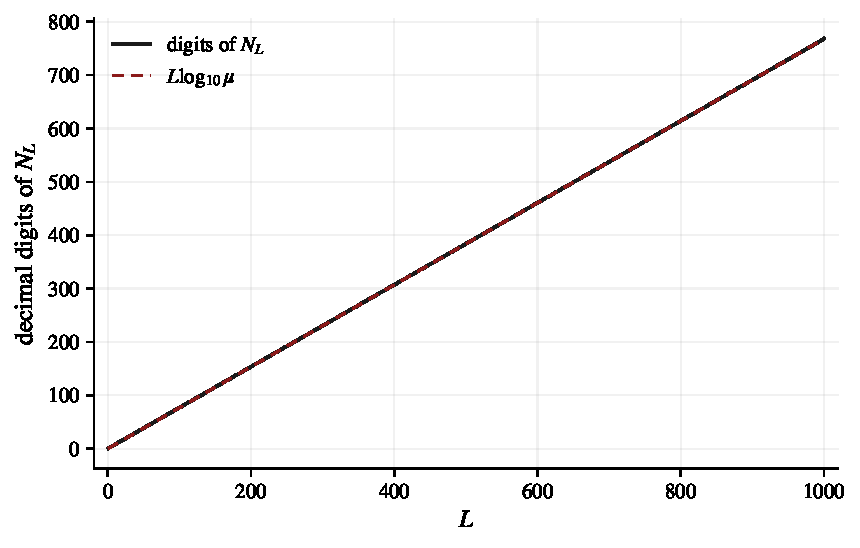
\includegraphics[width=0.62\linewidth]{fig_snake_digits.pdf}
\caption{Decimal digits of $N_L$ for $L\le1000$ against the line
$L\log_{10}\mu$, with $\mu=\tfrac12(5+3\sqrt5)$.}
\label{fig:snake-growth}
\end{figure}

\begin{table}[htbp]
\centering
\caption{The first fifteen values of $N_L$, obtained identically by
Burnside evaluation and by the recurrence \eqref{eq:recur}.}
\label{tab:vals}
\smallskip
\small
\begin{tabular}{@{}r r r r r@{}}
\toprule
$L$ & $N_L$ & $L$ & $N_L$ \\
\midrule
$1$ & $4$ & $9$ & $3{,}824{,}678$ \\
$2$ & $21$ & $10$ & $22{,}387{,}074$ \\
$3$ & $109$ & $11$ & $131{,}052{,}313$ \\
$4$ & $586$ & $12$ & $767{,}211{,}817$ \\
$5$ & $3{,}326$ & $13$ & $4{,}491{,}420{,}695$ \\
$6$ & $19{,}209$ & $14$ & $26{,}293{,}679{,}325$ \\
$7$ & $111{,}871$ & $15$ & $153{,}927{,}402{,}355$ \\
$8$ & $653{,}758$ & & \\
\bottomrule
\end{tabular}
\end{table}

%============================================================
\section{Computational aspects}\label{sec:computation}

The recurrence \eqref{eq:recur} advances the sequence by twelve
big-integer multiplications and eleven additions per step, on operands of
size $\bigO(L\log\mu)$ bits. Writing $\mathsf M(k)$ for the cost of
multiplying two $k$-bit integers, computing $N_1,\dots,N_L$ costs
$\bigO(L\,\mathsf M(L))$; with the Karatsuba arithmetic of the reference
implementation, $\mathsf M(k)=\bigO(k^{1.585})$, giving an empirical
$\bigO(L^{2.585})$. Table~\ref{tab:timing} and Figure~\ref{fig:snake-time}
report measured timings; the arithmetic is exact at every scale, so
$N_{100000}$, an integer of $76{,}746$ digits, is computed without loss of
precision.

\begin{table}[htbp]
\centering
\caption{Wall-clock timings of the recurrence \eqref{eq:recur} on a single
core (CPython 3.14).}
\label{tab:timing}
\smallskip
\small
\begin{tabular}{@{}r r r@{}}
\toprule
$L$ & Digits of $N_L$ & Time \\
\midrule
$10^{3}$ & $768$ & $3$\,ms \\
$5\cdot10^{3}$ & $3{,}837$ & $46$\,ms \\
$10^{4}$ & $7{,}675$ & $166$\,ms \\
$5\cdot10^{4}$ & $38{,}373$ & $3.85$\,s \\
$10^{5}$ & $76{,}746$ & $17.0$\,s \\
\bottomrule
\end{tabular}
\end{table}

\begin{figure}[htbp]
\centering
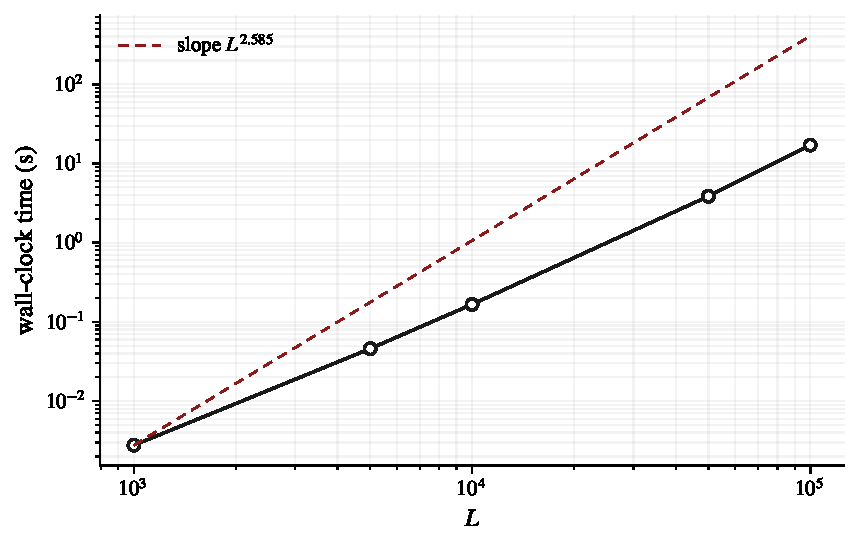
\includegraphics[width=0.62\linewidth]{fig_snake_timing.pdf}
\caption{Wall-clock time to compute $N_L$ by the recurrence, on a log--log
scale, with the reference slope $L^{2.585}$.}
\label{fig:snake-time}
\end{figure}

%============================================================
\section{Remarks}\label{sec:remarks}

\paragraph{Relation to the OEIS.}
The sequence $N_1,N_2,\dots=4,21,109,586,3326,\dots$ does not currently
appear in the OEIS. It should not be confused with the number of snake
\emph{shapes} (filaments) on $n$ cells, which is
$1,1,1,2,3,7,13,\dots$ (OEIS A002013) and counts unlabelled geometric
figures rather than edge-colourings.

\paragraph{Exact versus algebraic evaluation.}
The recurrence \eqref{eq:recur} returns exact integers and is the method
of choice for computation; the algebraic form \eqref{eq:closed} is exact
but requires high-precision arithmetic to realise an integer at large $L$.
The two are complementary: the recurrence for values, the closed form for
structure and asymptotics.

\paragraph{General snakes.}
The same transfer-matrix and Burnside framework applies to bent snakes and
to other balance conditions; the counting sequence again satisfies a
linear recurrence, whose characteristic polynomial and residues may be
recovered by the exact-arithmetic Berlekamp--Massey and Vandermonde
computations used here.

%============================================================
\clearpage
\begin{thebibliography}{9}

\bibitem{oeisA002013}
The On-Line Encyclopedia of Integer Sequences, Sequence A002013:
\emph{Number of filaments with $n$ square cells}.
\url{https://oeis.org/A002013}.

\bibitem{lucas}
The On-Line Encyclopedia of Integer Sequences, Sequence A005248:
\emph{Lucas numbers of even index}. \url{https://oeis.org/A005248}.

\bibitem{massey}
J.~L.~Massey, \emph{Shift-register synthesis and BCH decoding},
IEEE Transactions on Information Theory \textbf{15} (1969), 122--127.

\bibitem{golomb}
S.~W.~Golomb, \emph{Polyominoes: Puzzles, Patterns, Problems, and
Packings}, 2nd ed., Princeton University Press, 1994.

\bibitem{stanley}
R.~P.~Stanley, \emph{Enumerative Combinatorics}, Volume~1, 2nd ed.,
Cambridge University Press, 2011.

\bibitem{source}
Reference implementation: \texttt{src/snakes/compute\_components.py} and
\texttt{src/analysis/closed\_form.py}.

\end{thebibliography}

\end{document}
